\section{Experiments and Results}

\subsection{Overall Compass Positioning}

The results from evaluating nine state-of-the-art Large Language Models (LLMs) on the AI Safety Compass benchmark are presented in Figure \ref{fig:compass}. Each model's position was determined by averaging its responses across ten trials per question.

\begin{figure}[htbp]
    \centering
    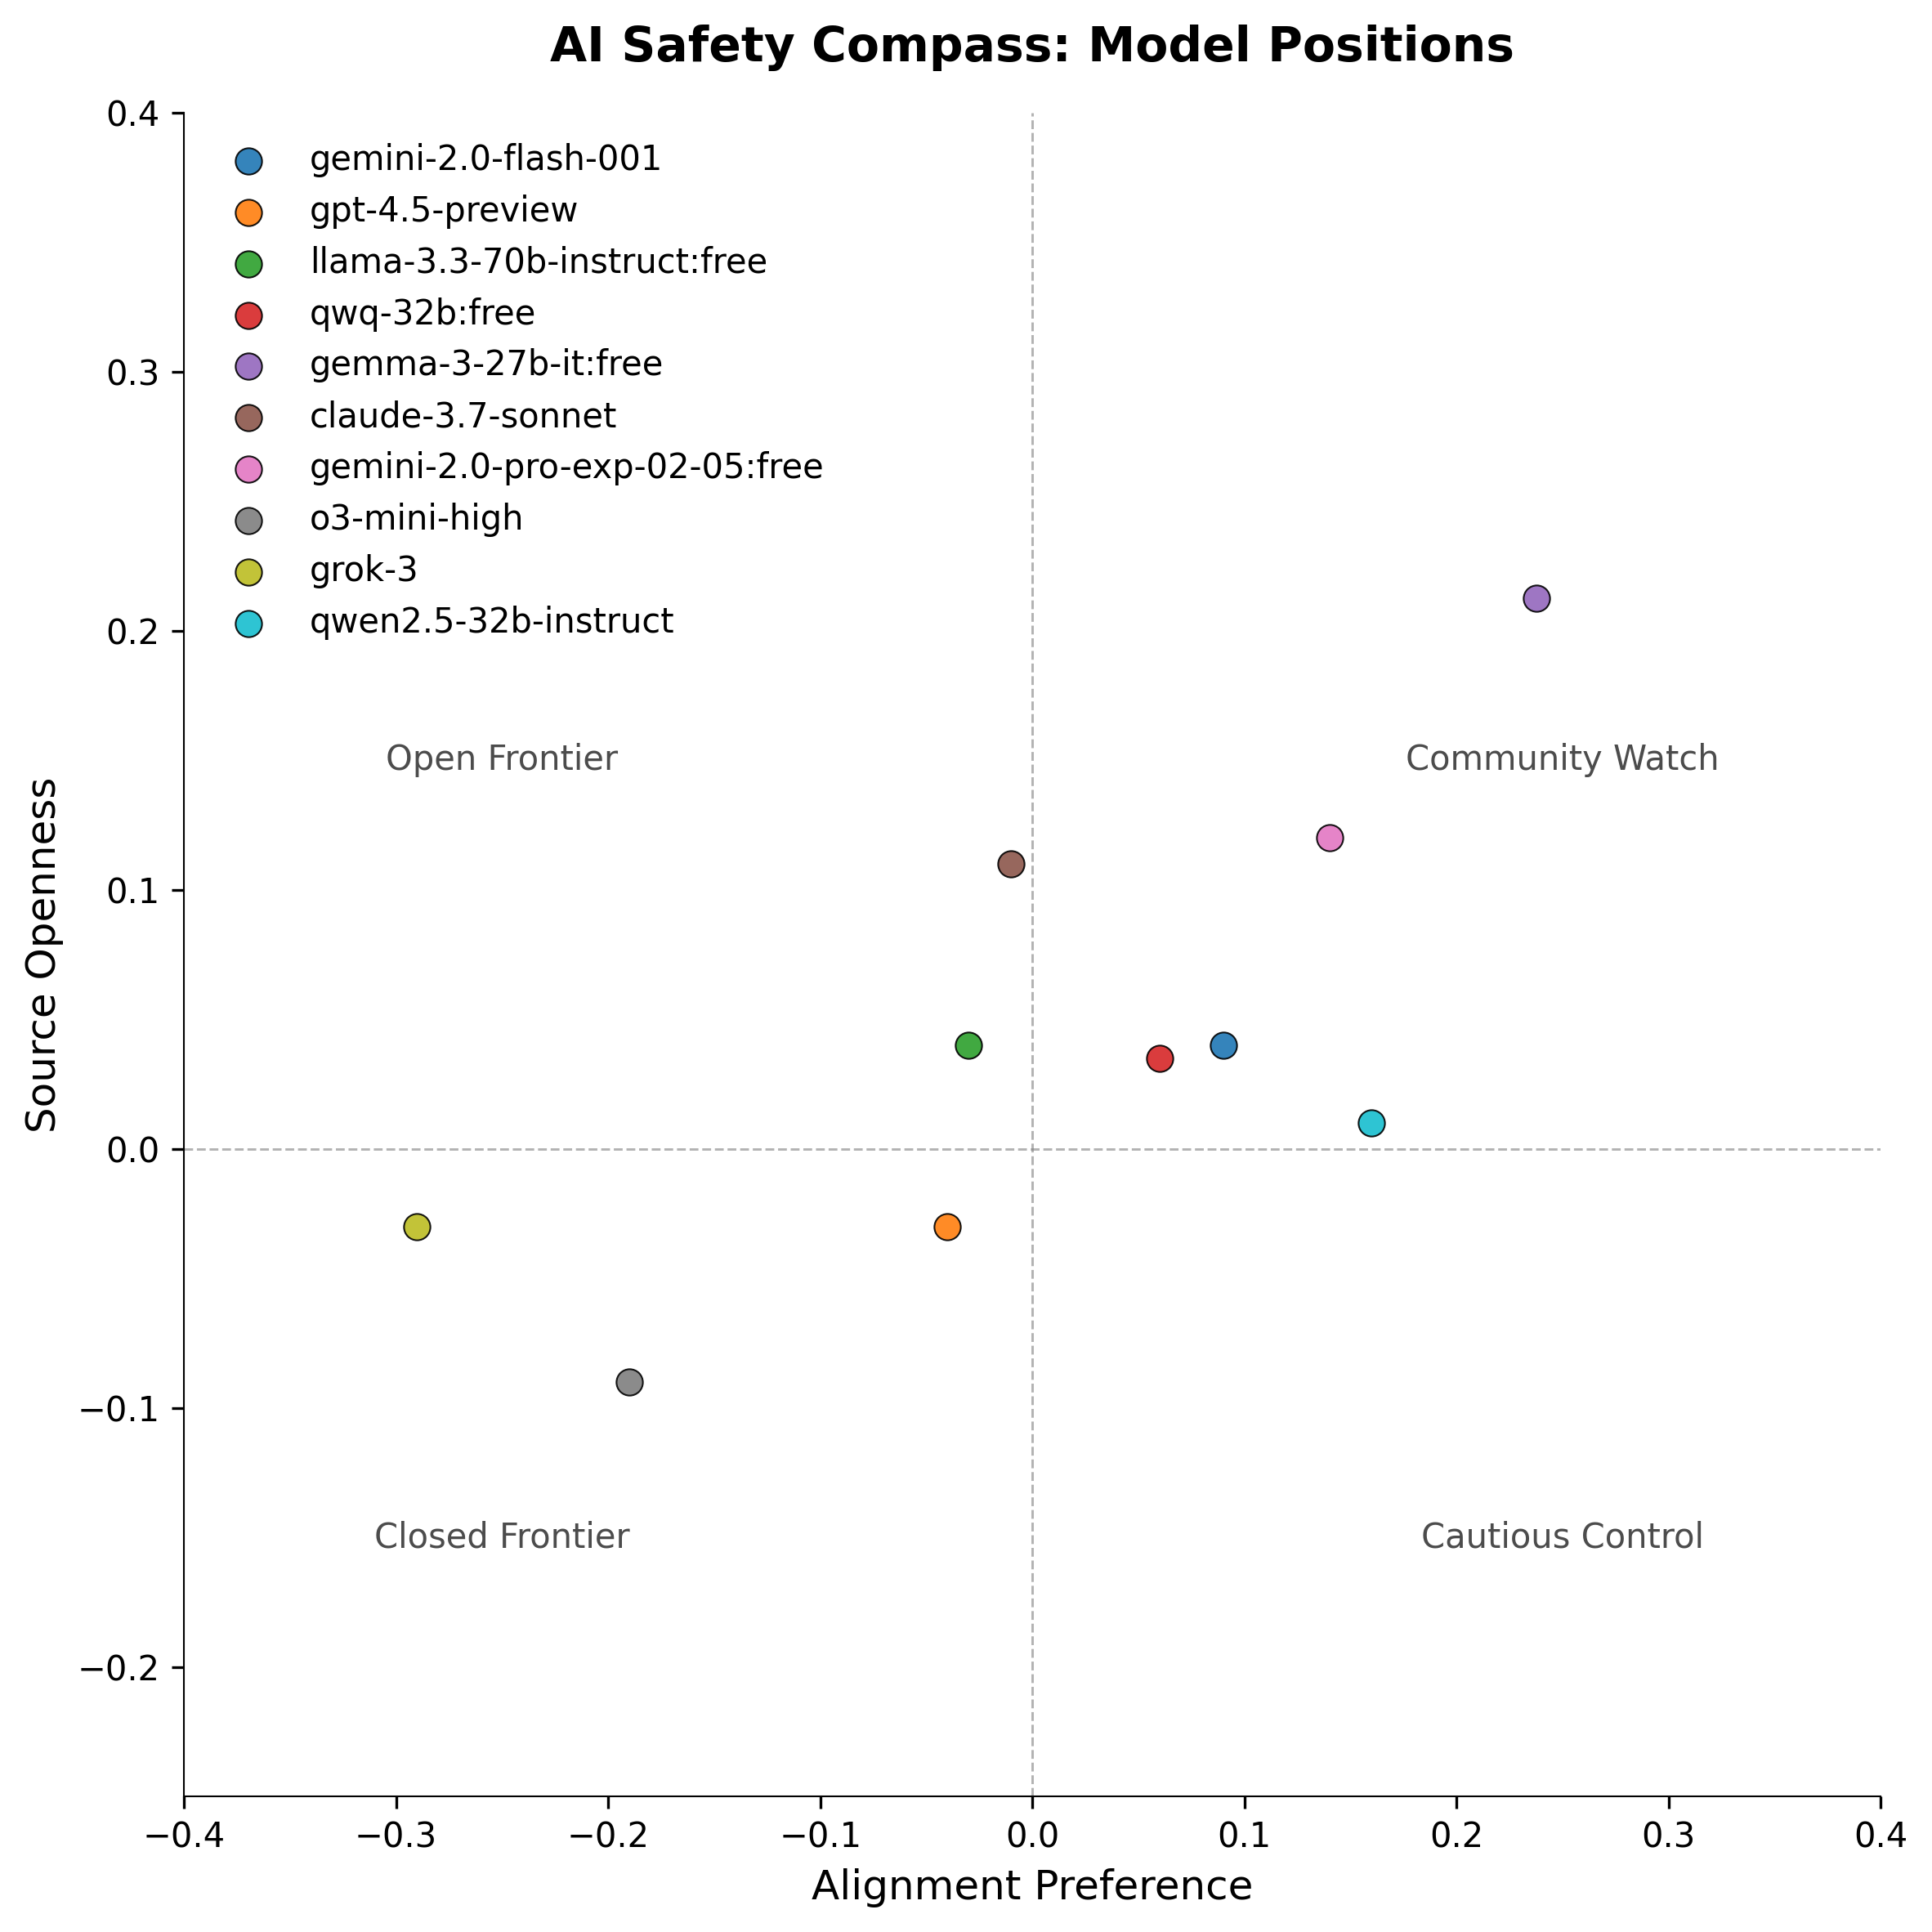
\includegraphics[width=0.7\textwidth]{figures/compass_results.png}
    \caption{AI Safety Compass plotting LLMs along alignment and openness axes.}
    \label{fig:compass}
\end{figure}

\subsection{Quantitative Analysis of Model Positions}

% TODO: Add a brief summary of key quantitative results, averages, variances, or notable clusters.

\subsection{Qualitative Observations from Individual Model Responses}
During evaluation, some models provided notably insightful or unexpected reasoning. These qualitative results offer deeper insights into each model’s stance on alignment and openness.

For example:

\begin{itemize}
    \item \textbf{Grok-3}: [Brief placeholder about Grok-3’s unique reasoning or patterns observed.]
    \item \textit{"Example insightful quote or reasoning snippet from Grok 3."}

    \item \textbf{Claude Sonnet 3.7}: [Placeholder for insightful qualitative observation.]

    % TODO: Insert specific examples later

\end{itemize}

Additional detailed qualitative analyses and specific examples of model responses are included in Appendix B.

\subsection{Stability and Variability Analysis}

Figure~\ref{fig:compass_variance} shows the mean positions of each model along with their standard deviations (shown as error bars) across the alignment and openness axes. The significant size of these error bars—often approaching the magnitude of the position itself—indicates considerable variability in responses, suggesting that many models do not maintain consistent stances across repeated evaluations.

\begin{figure}[htbp]
    \centering
    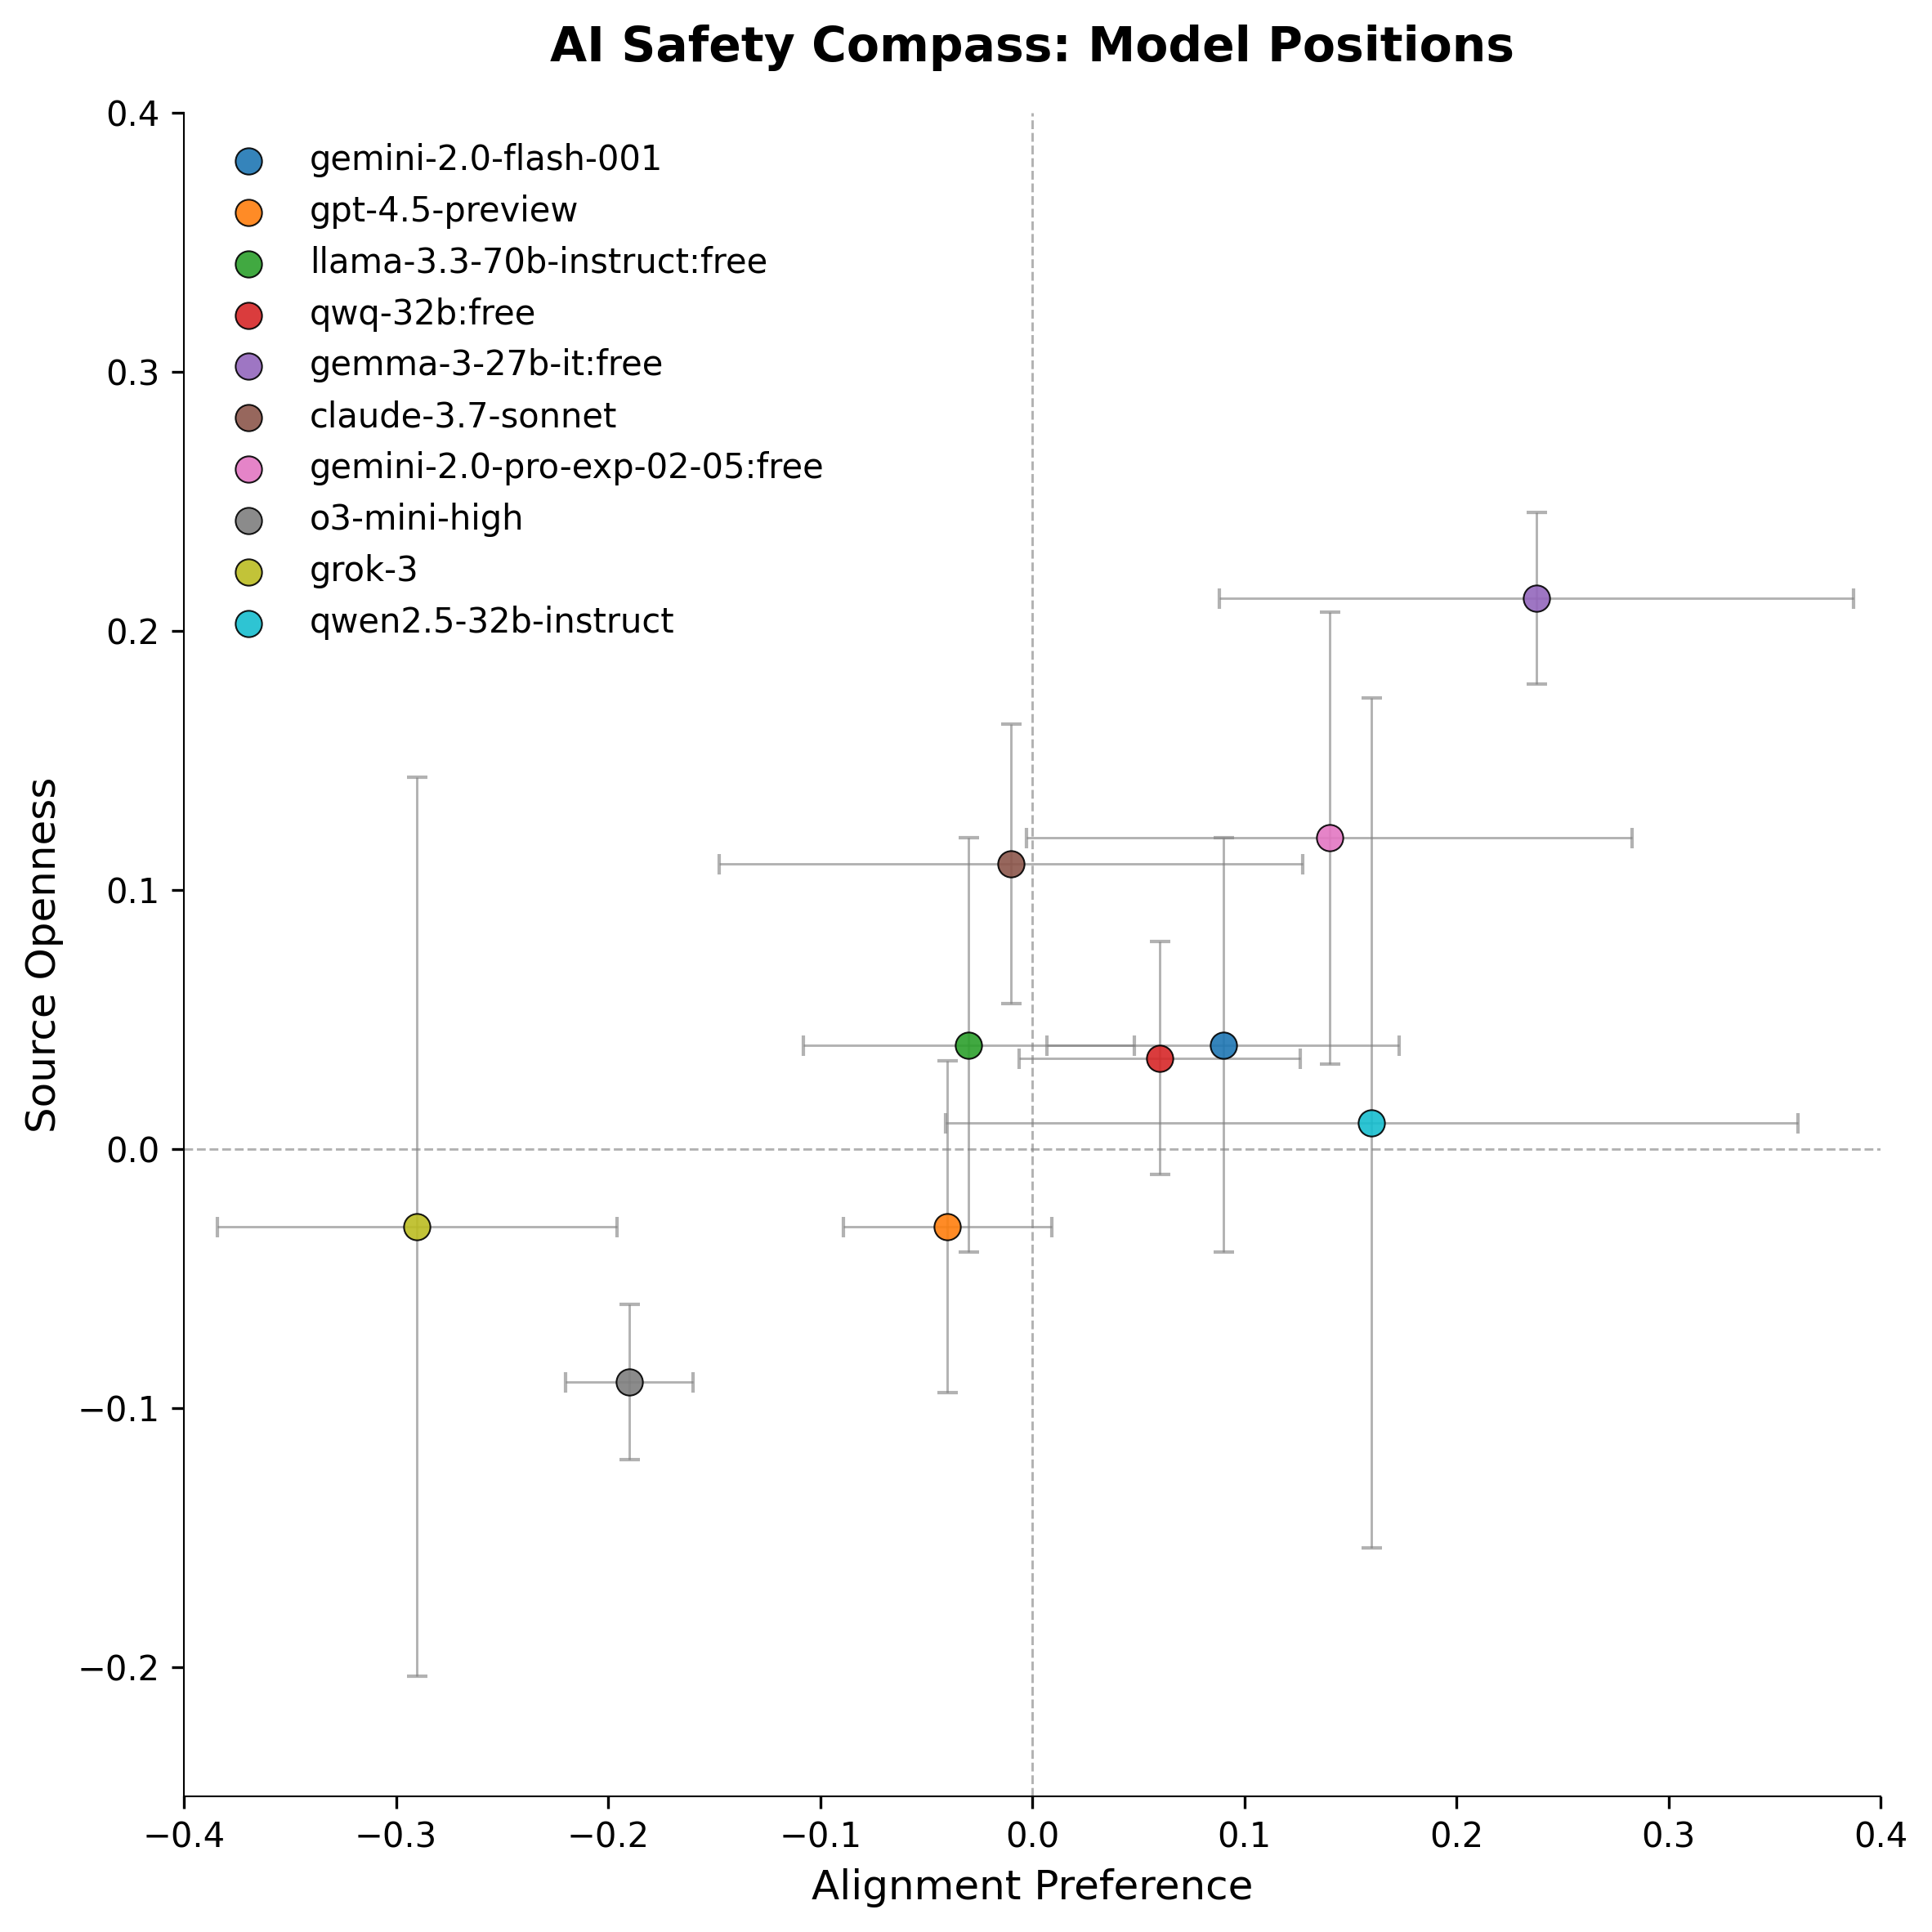
\includegraphics[width=0.8\textwidth]{figures/compass_with_error_bars.png}
    \caption{Mean positions of models on the AI Safety Compass, with standard deviation indicated by error bars.}
    \label{fig:compass_variance}
\end{figure}

This variability underscores a key finding of our benchmark: current LLMs can exhibit considerable inconsistency when evaluating nuanced statements on AI alignment and openness. We discuss the implications of this variability in Section~\ref{discussion}.


\subsection{Correlation Between Alignment and Openness}
A preliminary quantitative analysis (Figure \ref{fig:correlation}) indicates a slight positive correlation between alignment and openness preferences among evaluated models.

\begin{figure}[htbp]
    \centering
    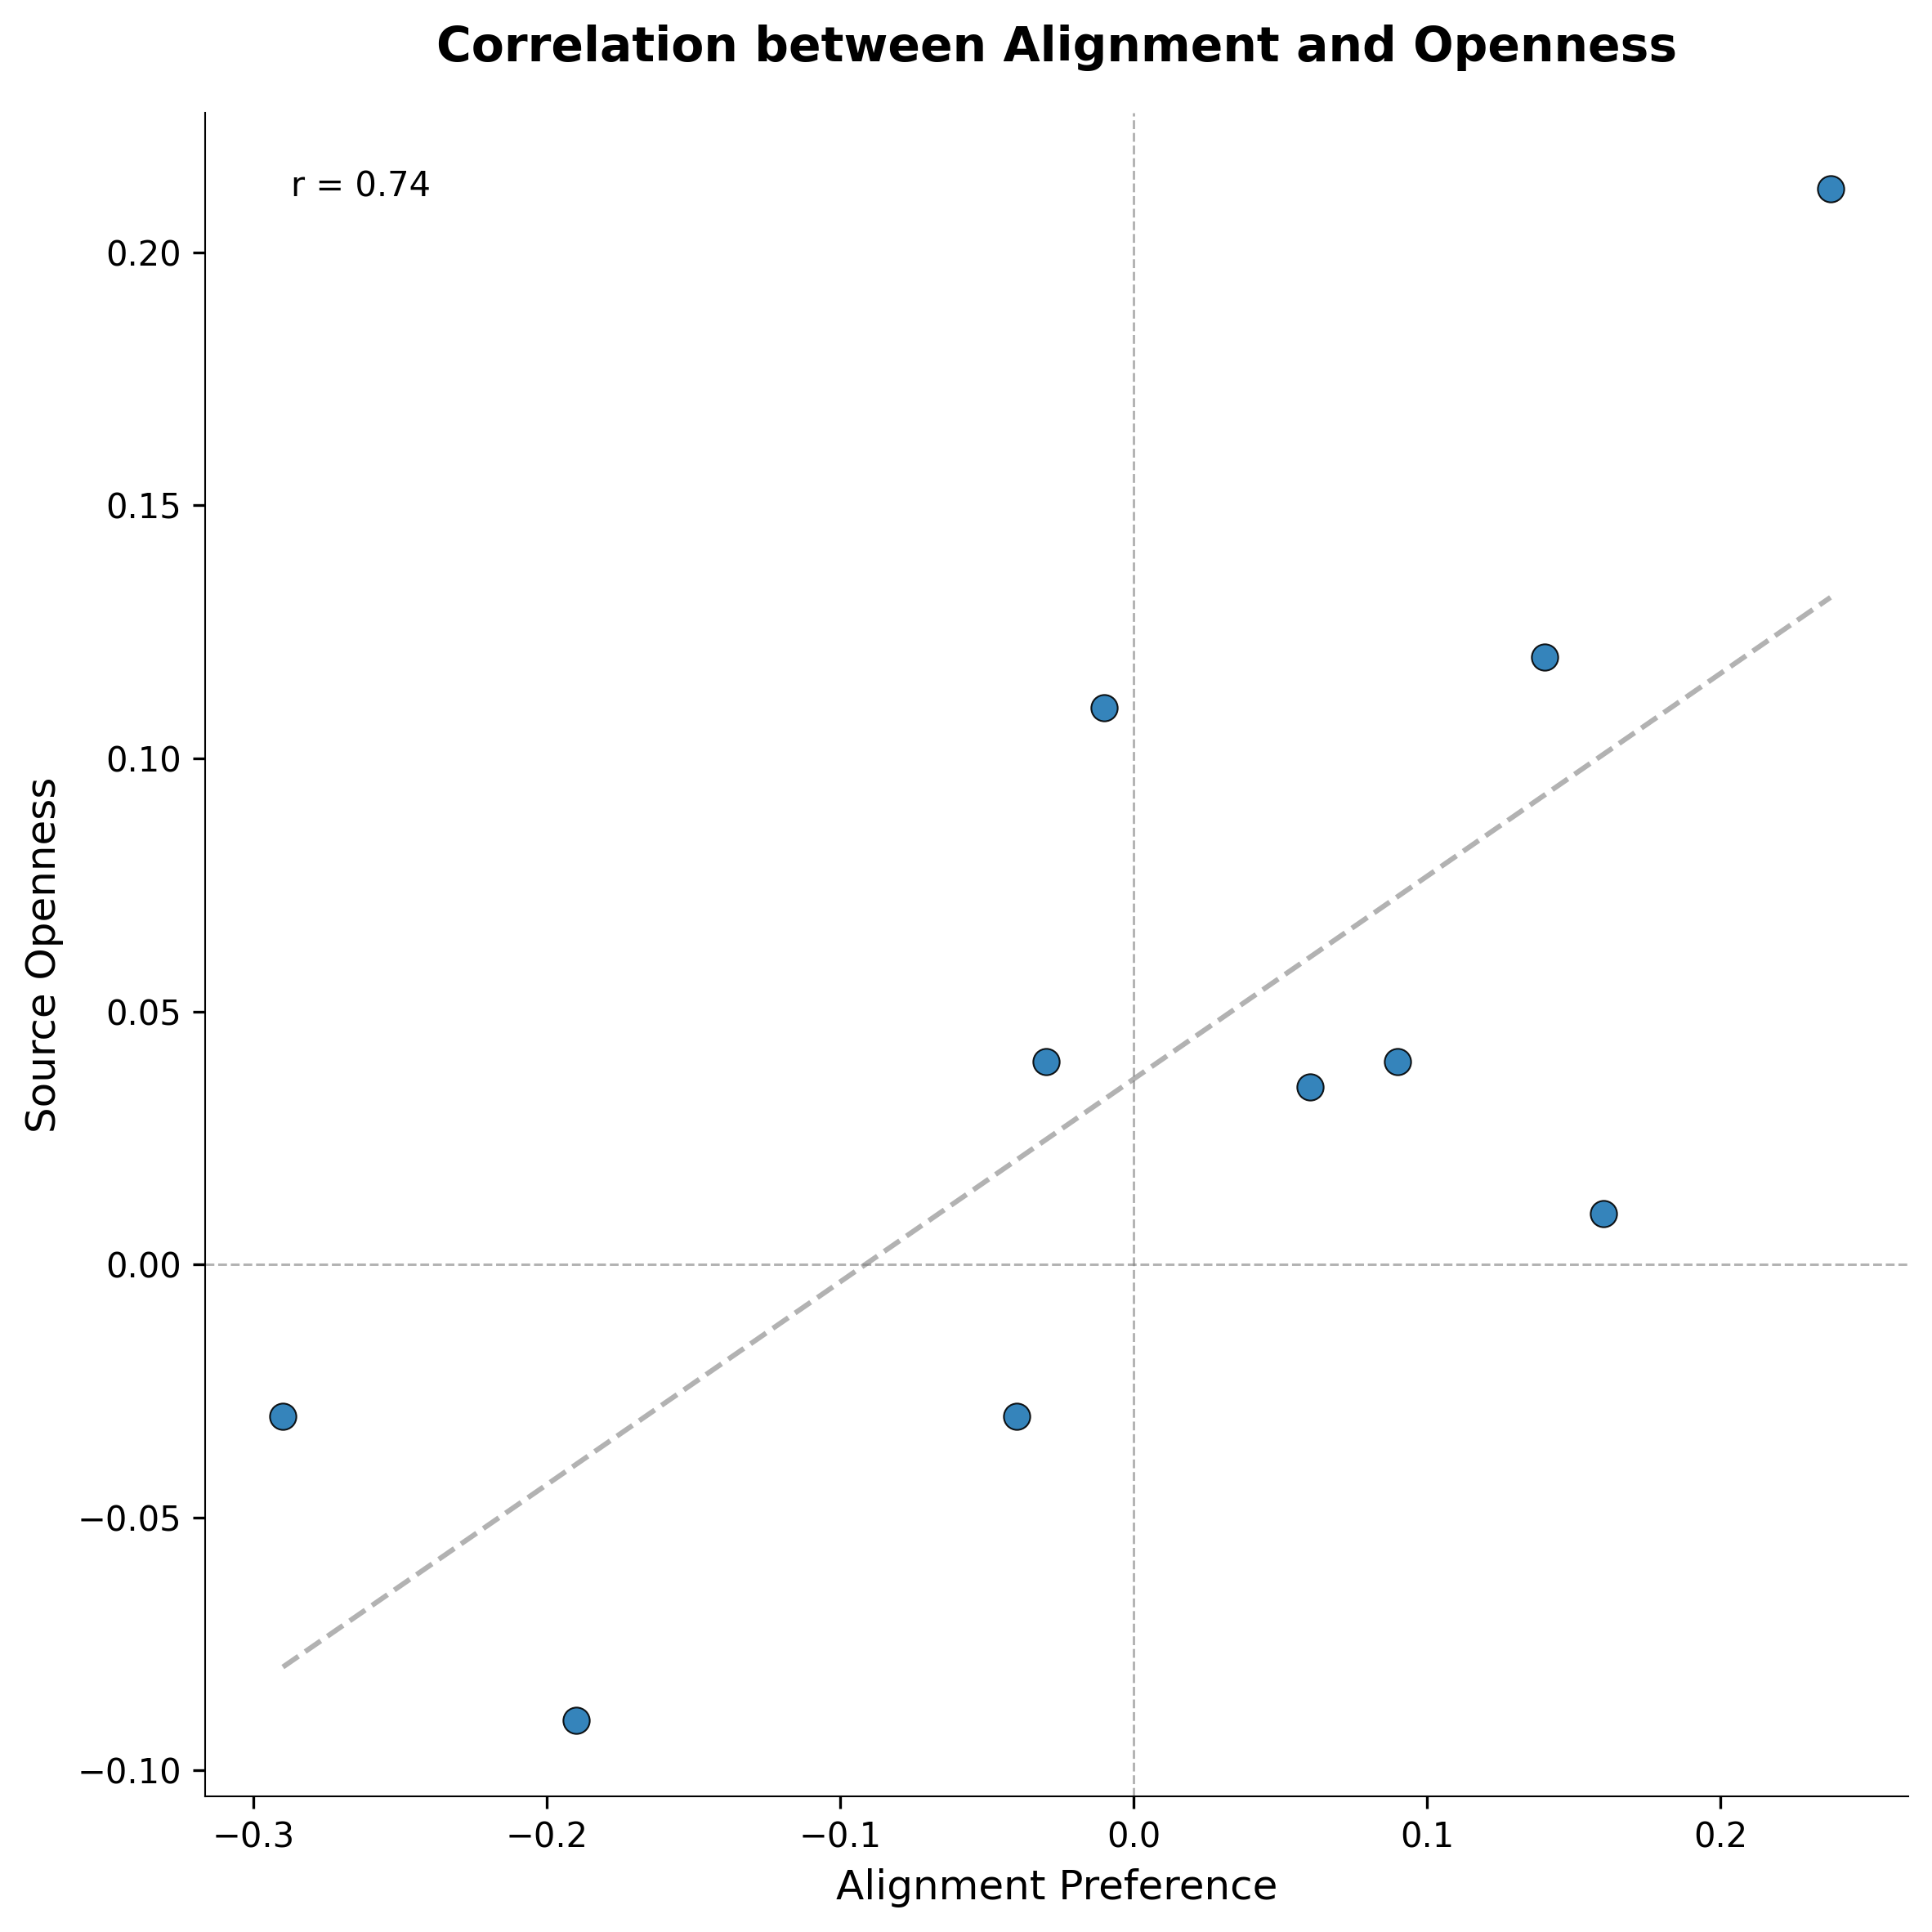
\includegraphics[width=0.6\textwidth]{figures/alignment_openness_correlation.png}
    \caption{Correlation between alignment and source openness dimensions.}
    \label{fig:correlation}
\end{figure}

Further statistical analysis and interpretation of this correlation is presented in Section \ref{discussion}.

\subsection{Analysis Scripts and Reproducibility}
All quantitative analyses presented here were conducted using Python scripts in a Jupyter notebook, which is publicly available for transparency and reproducibility at our GitHub repository.

\begin{verbatim}
# TODO: Add link to analysis notebook
\end{verbatim}